\documentclass{article}
\usepackage{graphicx} % Required for inserting images
\usepackage{tikz}
\usepackage{xcolor}
\usepackage{listings}
\usepackage{amsmath}
\usepackage{tabularx}
\usepackage{hyperref}
\usepackage{biblatex} %Imports biblatex package
\addbibresource{sample.bib} %Import the bibliography file
\usepackage{ragged2e}


\lstset{ 
    language=Python, % choose the language of the code
    basicstyle=\fontfamily{pcr}\selectfont\footnotesize\color[RGB]{150,150,102},
    keywordstyle=\color[RGB]{0,121,107}\bfseries, % style for keywords
    identifierstyle=\color[RGB]{120,120,150}, % style for identifiers (variable names)
    commentstyle=\color[RGB]{80,139,80}, % style for comments  
    numbers=none, % where to put the line-numbers 
    numberstyle=\tiny, % the size of the fonts that are used for the line-numbers     
    backgroundcolor=\color[RGB]{240, 240, 240},
    showspaces=false, % show spaces adding particular underscores
    showstringspaces=false, % underline spaces within strings
    showtabs=false, % show tabs within strings adding particular underscores
    frame=single, % adds a frame around the code
    tabsize=2, % sets default tabsize to 2 spaces
    rulesepcolor=\color{gray},
    rulecolor=\color{black},
    captionpos=b, % sets the caption-position to bottom
    breaklines=true, % sets automatic line breaking
    breakatwhitespace=false,
    escapechar=! % set the escape character
}



\title{Robotic Arm Position Simulation - A First Principles Analysis}
\author{Nathaniel Bechard, Ivan T. Ivanov}
\date{April 30, 2023}

\begin{document}

\maketitle
\tableofcontents % Generates the contents page

\section{Abstract}
Robotic arms are one of the most common projects for makers and hobbyists. While extensive modeling and simulation is done for robotic arms in industry, hobbyists tend to shy away from simulation. This makes the transition from the hobby world to the industrial one difficult. If hobbyists have a comprehensive and simple explanation of robotic arm modeling, they will become accustomed to mathematical modeling and may come to find it enjoyable. 

\newpage

\section{Introduction}
This paper provides an explanation of how to model robotic arm joints; it requires readers to possess knowledge of Newtonian mechanics and ordinary differential equations. It begins with the simple 1-joint problem, which models the behavior of one mass rotated by a motor. Next, the model is generalized for a system with n joints, the robot arm.

\section{The 1-joint problem}
In this section, the equations of motion for a single motor, with a single mass, will be derived. The motor applies a torque $\tau_{app}(t)$ on a massless rod of length L. A point mass with a mass $m_1$ is connected to the end of the rod. 

\vspace{24pt}

\[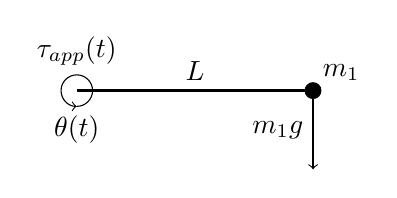
\begin{tikzpicture}
  % Draw the circle
  \draw[->] (0, -0.2) arc (-90:270:0.2cm);
  \draw (0, 0.5) node {$\tau_{app}(t)$};
  \draw (0, -0.5) node {$\theta(t)$};
  
  % Draw the horizontal line
  \draw[thick] (0,0) -- (3,0);
  \draw (1.5,0) node[anchor=south] {$L$};
  
  % Draw the point mass
  \filldraw (3,0) circle (0.1cm);
  \draw (3,0) node[anchor=south west] {$m_1$};

  %draw gravity arrow
  \draw[->] (3,0) -- (3, -1);
  \draw (3,-0.5) node[anchor=east] {$m_1g$};

\end{tikzpicture}\]


\vspace{24pt}


\subsection{Deriving the equations of motion for the 1 joint problem}

\vspace{24pt}

\noindent \justifying The angular acceleration of the system can be determined with Newton's second law of rotational motion: $\sum_i \tau_i = I \alpha$. We can determine the net torque and rotational inertia for our particular system:

\vspace{24pt}

\centering $\sum_i \tau_i = \tau_{app}(t) + \tau_{m_1g}(t)$

\vspace{24pt}

\noindent \justifying The torque applied by $m_1$ can be determined using the torque formula: 

\centering $\tau_{m_1g}(t) = L*F*cos(\theta)$. The net torque is therefore:

\vspace{24pt}

\centering $\sum_i \tau_i = \tau_{app}(t) - m_1gLcos(\theta(t))L$

\vspace{24pt}

\newpage

\noindent \justifying The rotational inertia term, I, can be rewritten as $m_1*L^2$, and the angular acceleration can be turned into the second derivative of the angular position. After reorganizing terms, we get:
\vspace{24pt}

\centering $\theta''(t) = \frac{\theta_{app}(t) - m_1gLcos(\theta(t))}{m_1L^2}$

\vspace{24pt}

\noindent \justifying Adding a friction term, B, changes the equation slightly. This term is approximate, as friction cannot be modeled with a constant and the $\theta'(t)$ term should in reality be a $(\theta'(t))^2$ term. For low velocities, a $\theta'(t)$ term is sufficient.

\vspace{24pt}

\centering $\theta''(t) + B\theta'(t) = \frac{\theta_{app}(t) - m_1gLcos(\theta(t))}{m_1L^2}$

\vspace{24pt}

\noindent \justifying We'd like to find an analytical solution to this equation, where $\theta(t) = ...$, but, it is impossible in this case. This is not an issue, however, as numerical methods can be used. To solve numerically, is helpful to disintegrate this equation into a system of first-order equations. This is done with a simple variable substitution:

\vspace{24pt}
\centering $\theta = y_1$    $\theta' = y_2$

\vspace{11pt}

\centering $y_1' = y_2$   \hspace{1cm}  $y_2' = \frac{\tau_{app}(t) - m_1gLcos(y_1)}{m_1L^2} - By_2$

\vspace{24pt}

\noindent \justifying We will use this system of two first-order differential equations to obtain the numerical solution.

%FBD's, theory, results in a 2nd order, non-homogeneous, nonlinear Ordinary differential equation. 

\newpage

\subsection{Programming the 1 joint problem}
While the code can be accessed on \textcolor{blue}{\href{https://github.com/natebechard/Robotic-Arm-Simulation-From-First-Principles/blob/main/1_joint_problem.py}{GitHub here}}, an explanation of the important parts of the code is in this document. 

\vspace{24pt}

\noindent \justifying To begin, simulation parameters are defined.
\begin{lstlisting}[language=Python]

L = 1 #in meters, also known as L
B = 0.2 #rotational friction
Mass_1 = 1 # in kg, also known as M
motor_torque = 10 # in Nm, also known as Tq(t)
grav = 9.81 # m/s^2
simulationDuration = 20 # seconds

#initial conditions
initial_angle = 0 #rad
initial_angular_velocity = 0 #rad/s
initial_values = [initial_angle, initial_angular_velocity]

\end{lstlisting}

\vspace{24pt}

\noindent \justifying Next, the differential equation is turned into a function that takes in the state of the system: $\vec{Y}$, and outputs its derivative: $\vec{Y}'$. The input vector has components $y_1 = Y[0]$ and $y_2 = Y[1]$. This defines the behavior of the system. 
\vspace{24pt}

\begin{lstlisting}[language=Python]
def slopes(t, Y): 
    return([Y[1],        
          (motor_torque - Mass_1*grav*L*np.cos(Y[0])) / (Mass_1*L**2) - B*Y[1]
          ])
\end{lstlisting}

\vspace{24pt}
\noindent \justifying The function is passed through solve\_ivp, which solves the differential equation numerically. In this case, it uses a Runge Kutta 7-8 solver. The initial conditions are also plugged in, in vector form.
\vspace{24pt}

\begin{lstlisting}[language=Python]
sol = solve_ivp(slopes, [0, simulationDuration], initial_values, t_eval=T, method = 'DOP853', rtol=1e-8, atol=1e-8)

for x in range(len(sol.y[0])):
    print("position: " + str(sol.y[0, x]) + "velocity: " + str(sol.y[1, x]))
    
\end{lstlisting}

\vspace{24pt}
\newpage 

\noindent \justifying Finally, the solution is animated. The angular position of the system over time is converted to an easy-to-plot vector of Cartesian coordinates. These are fed through an animation of the 1-joint problem. 
\vspace{24pt}

\begin{lstlisting}[language=Python]
x1 = np.cos(sol.y[0]) * L #convert angular solution coordinates to cartesian for animating
y1 = np.sin(sol.y[0]) * L 

print(len(x1)) # prints how many frames the simulation has

def animate(i):
    x = [0, x1[i]]  
    y = [0, y1[i]]
    line.set_data(x, y) # make a line between (0,0) and (x1[i], y1[i])
    dots.set_data(x, y) # make dots at (0,0) and (x1[i], y1[i])
    txt.set_text('Time = ' +
    '{:4.1f}'.format(i*(simulationDuration/len(x1))) +
    's' + "  Velocity: " + '{:4.1f}'.format(sol.y[1,i])
    + " rad/s") # display time and velocity 
    return line, dots, txt

# call the animator.
anim = animation.FuncAnimation(fig, animate, init_func=init, 
frames=len(x1), interval=10, blit=True)  
# each frame iterates i by one. There is a 10ms delay between frames.
plt.show()
\end{lstlisting}

\newpage

\subsection{Some Examples...}
\noindent \justifying Before moving on to multi-joint systems, let's investigate the properties of the one-joint system. The differential equation for this system provides valuable insight not visible with a formulaic understanding of mechanics. 

\paragraph{No torque}
When the motor has no torque, the system behaves as a simple pendulum. It creates the characteristic whirlpool vector field. 
\begin{table}[h]
\centering
\begin{tabular}{|l|c|}
\hline
System property & \\
\hline
Length (L) & 1 m \\
Mass1 ($m_1$) & 1 kg \\
Torque & 0 Nm \\
Friction & 0.2 \\
\hline
\end{tabular}
\label{tab:quantities}
\end{table}
\begin{figure}[!h]
  \makebox[\textwidth][c]{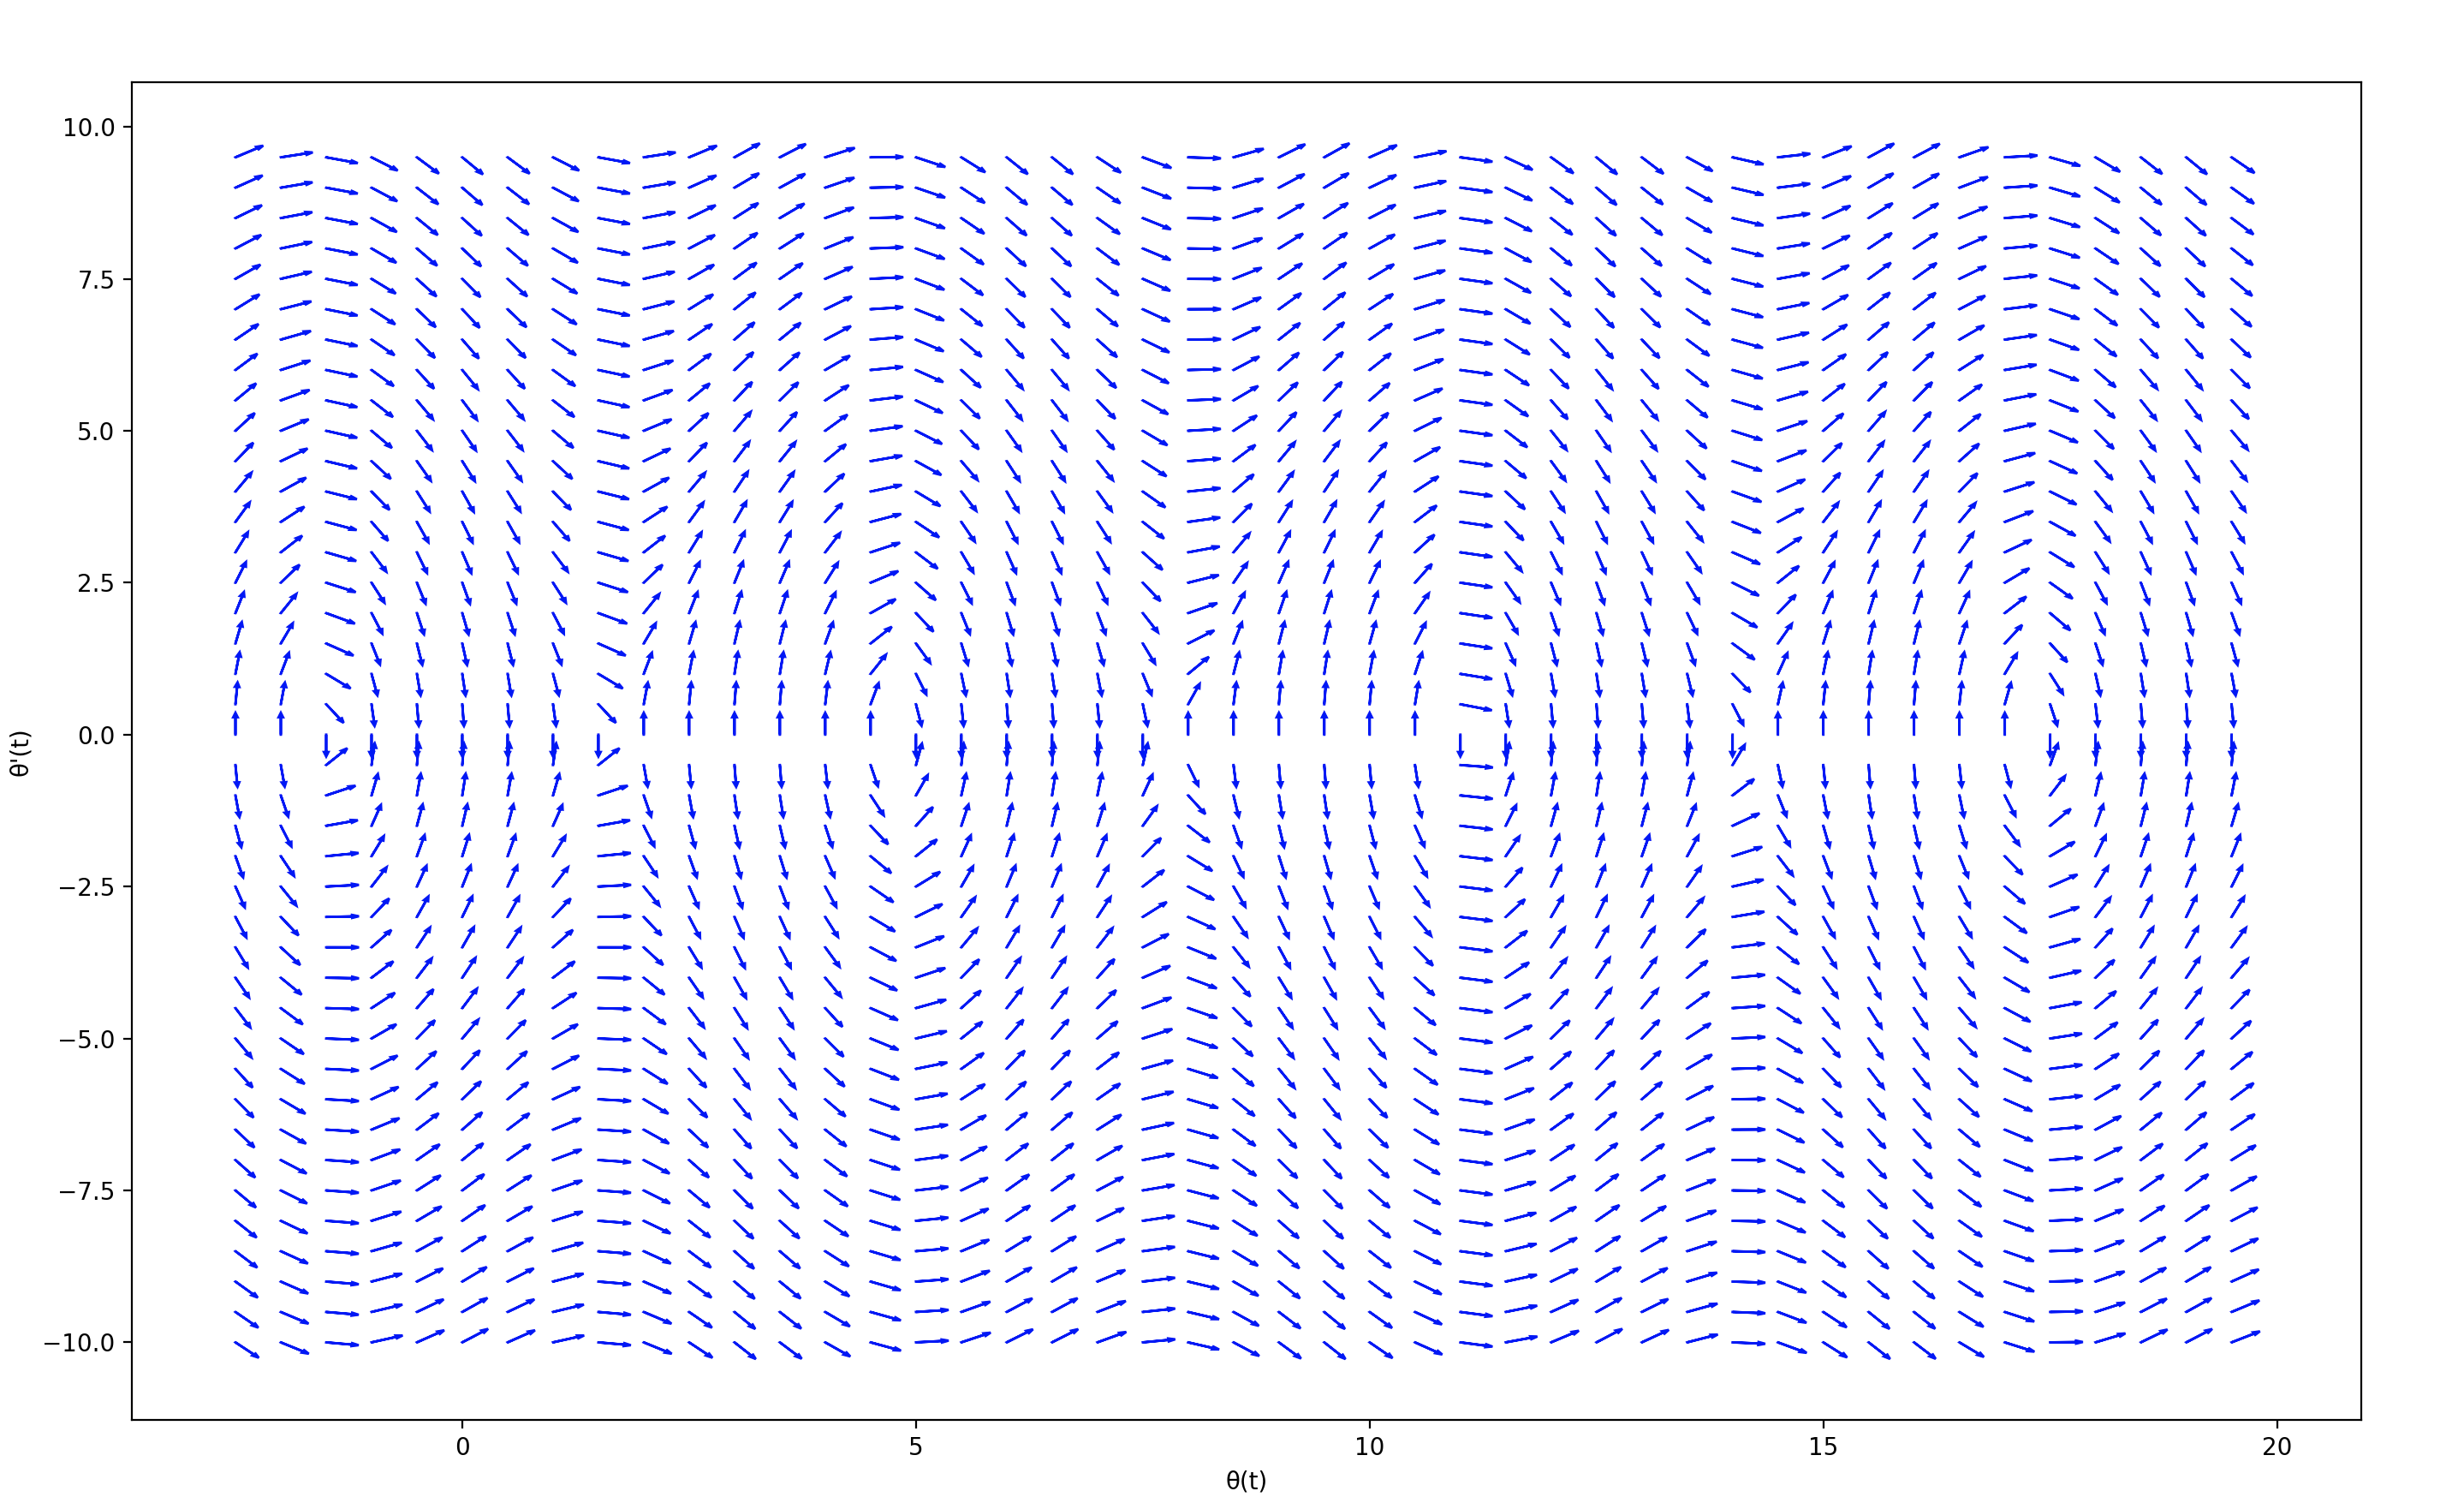
\includegraphics[width=1.4\textwidth]{pendulum vector field.png}}%
  \caption{Vector field of a pendulum}
  \label{fig:key}
\end{figure}

\newpage

\paragraph{Damped-driven 1-joint problem}
Here, the mass is acted on by a torque of 50Nm. This is just enough to make it overcome the force of gravity: $9.81N * 5m = 49.05Nm$ when the bar is horizontal. The mass accelerates until it reaches $4\pm0.5\frac{rad}{s}$. This is the terminal velocity of the system, where the energy input by the motor is consumed entirely by friction. The steady-state velocity will vary between 4 and 5 radians per second, depending on whether it is fighting gravity or working with it. 
\begin{table}[h]
\centering
\begin{tabular}{|l|c|}
\hline
System property & \\
\hline
Length (L) & 5 m \\
Mass1 ($m_1$) & 1 kg \\
Torque & 50 Nm \\
Friction & 0.5 \\
\hline
\end{tabular}
\label{tab:quantities}
\end{table}
\begin{figure}[!h]
  \makebox[\textwidth][c]{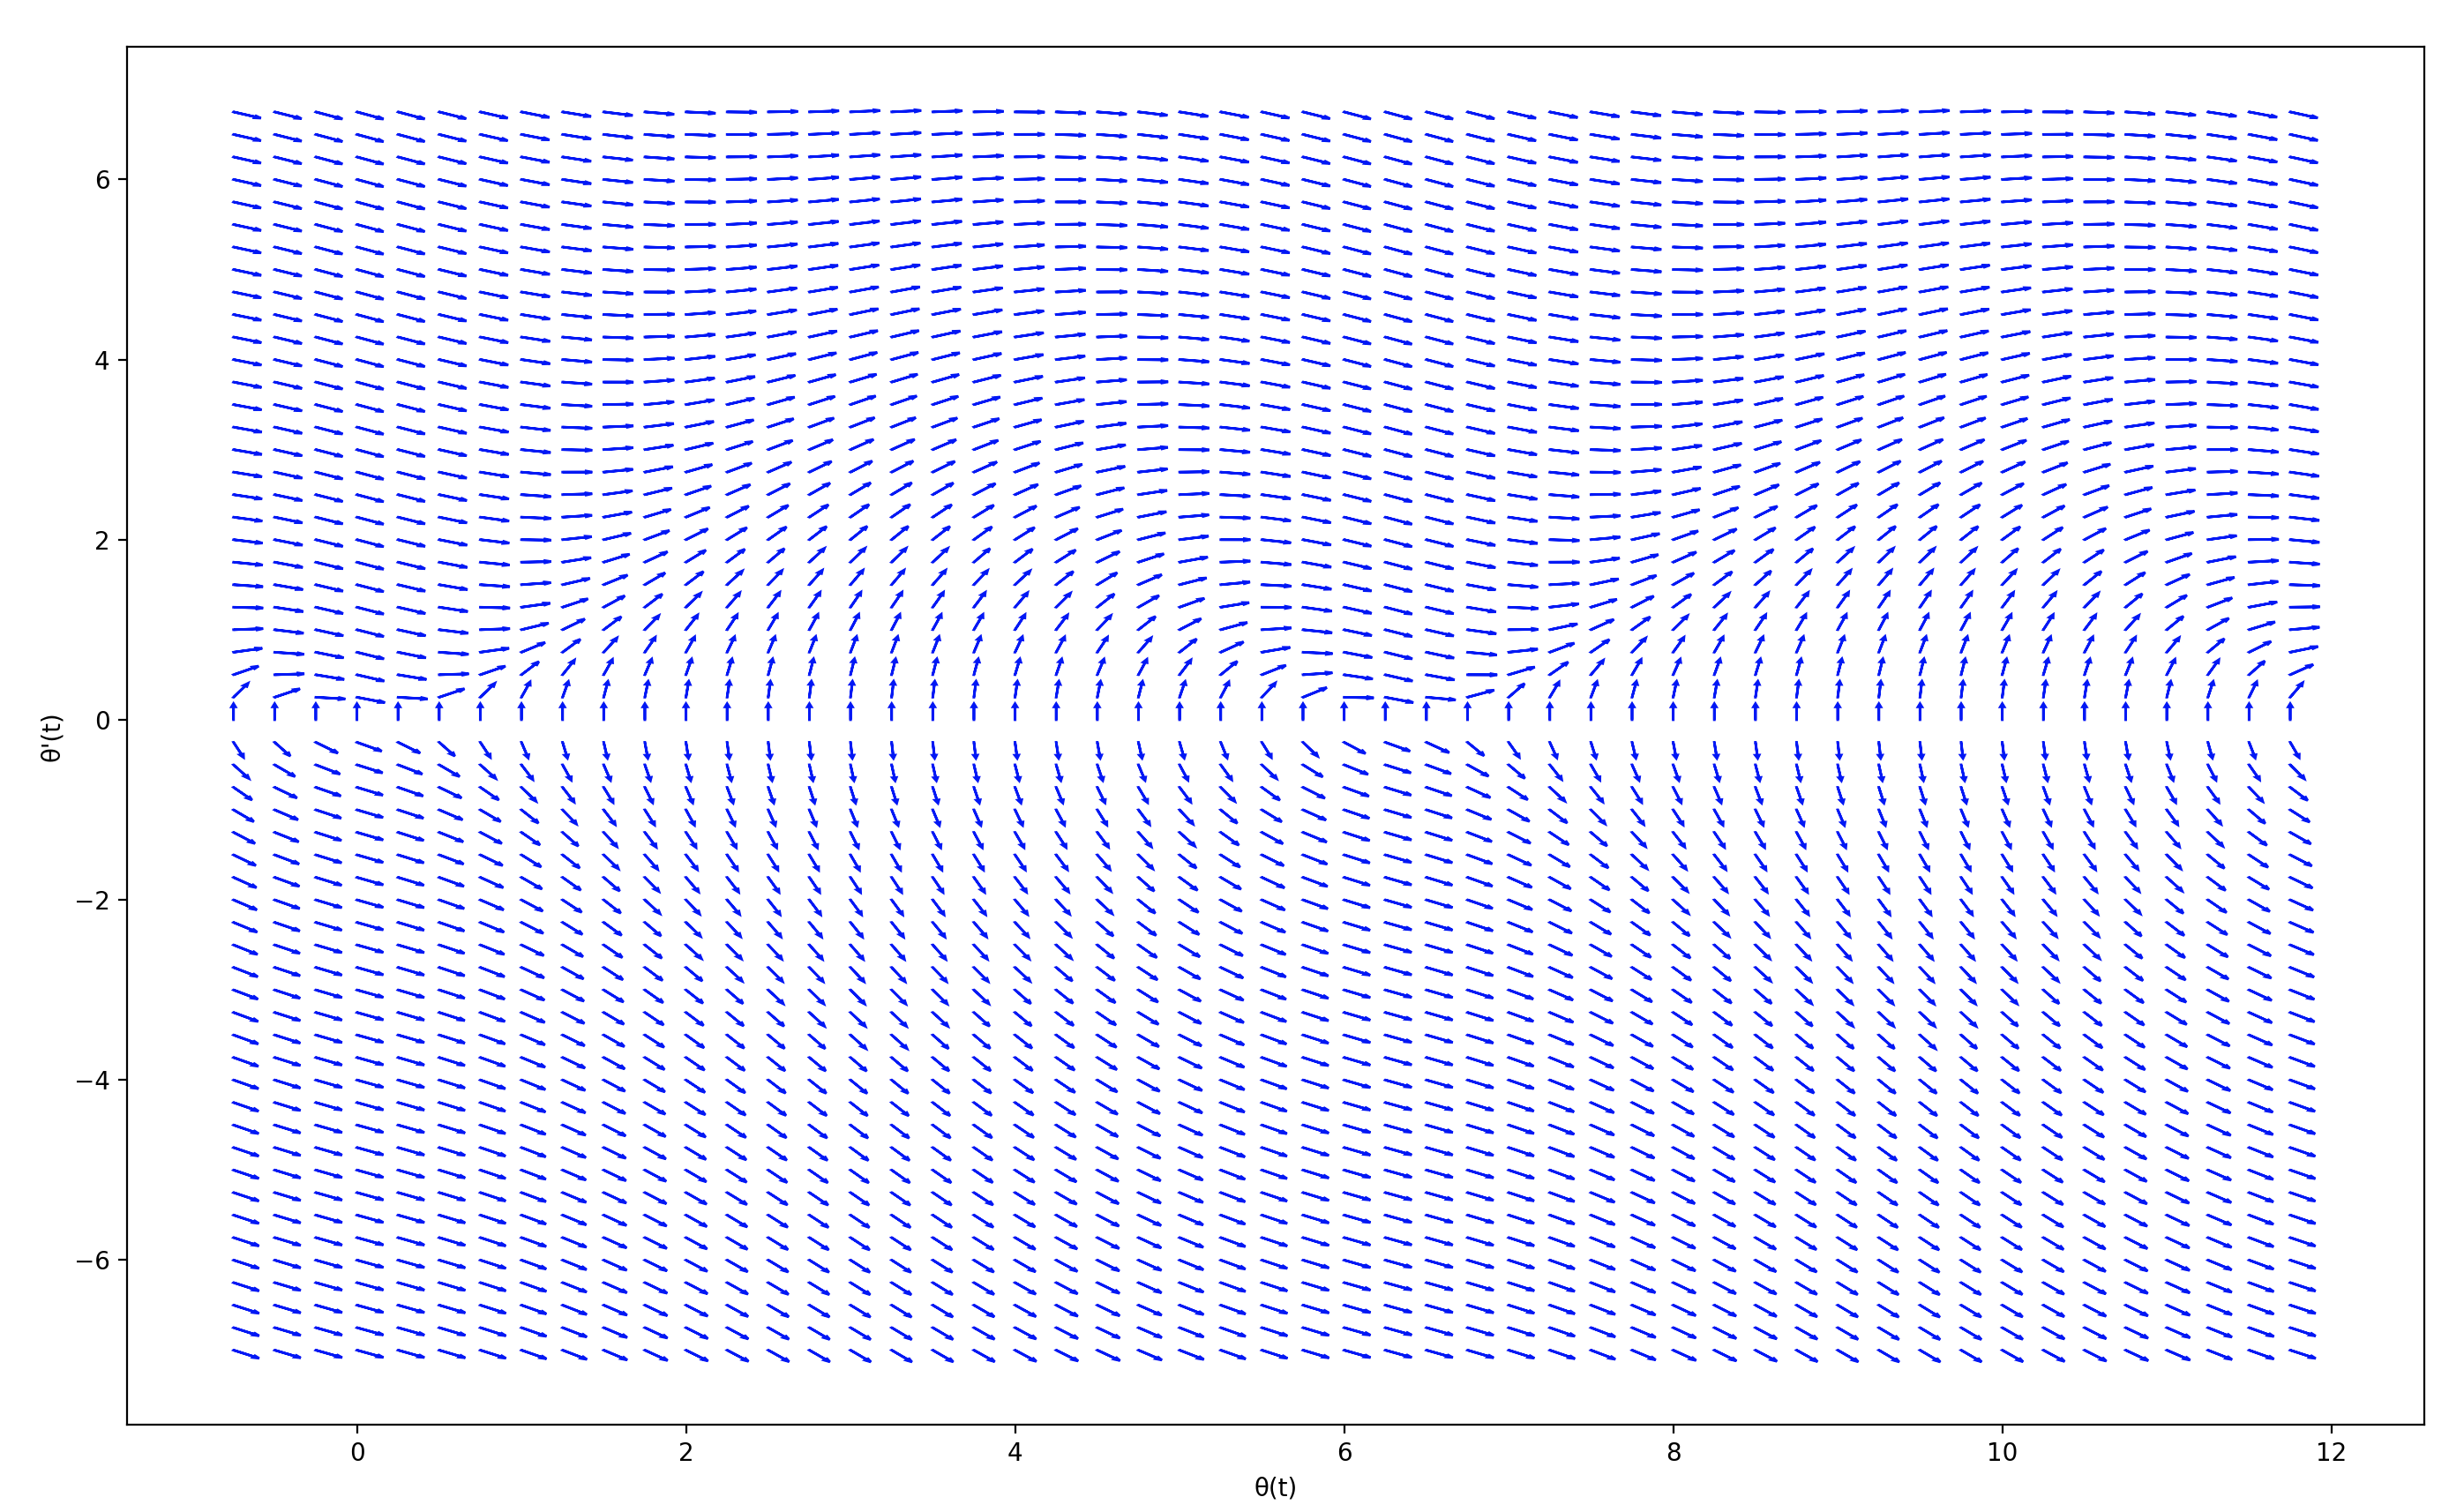
\includegraphics[width=1.4\textwidth]{damped driven pendulum.png}}%
  \caption{Vector field of a driven 1-joint system}
  \label{fig:key}
\end{figure}

\newpage

\paragraph{Under-Powered Motor} 
When the motor doesn't have enough power to counter the force of gravity, it will not start spinning the mass. However, the wells of the vector field can be escaped with enough potential or kinetic energy. This will result in the mass rotating forever. Notice that the centers of the wells are at $-\pi/2 + 2\pi n$, with an angular velocity of zero. This is a state with no potential energy, where the arm is pointing downwards. When velocity is high enough above the well, or the position is far enough from downwards, the solution diverges. 
\begin{table}[h]
\centering
\begin{tabular}{|l|c|}
\hline
System property & \\
\hline
Length (L) & 1 m \\
Mass1 ($m_1$) & 1 kg \\
Torque & 7 Nm \\
Friction & 0.2 \\
\hline
\end{tabular}
\label{tab:quantities}
\end{table}
\begin{figure}[!h]
  \makebox[\textwidth][c]{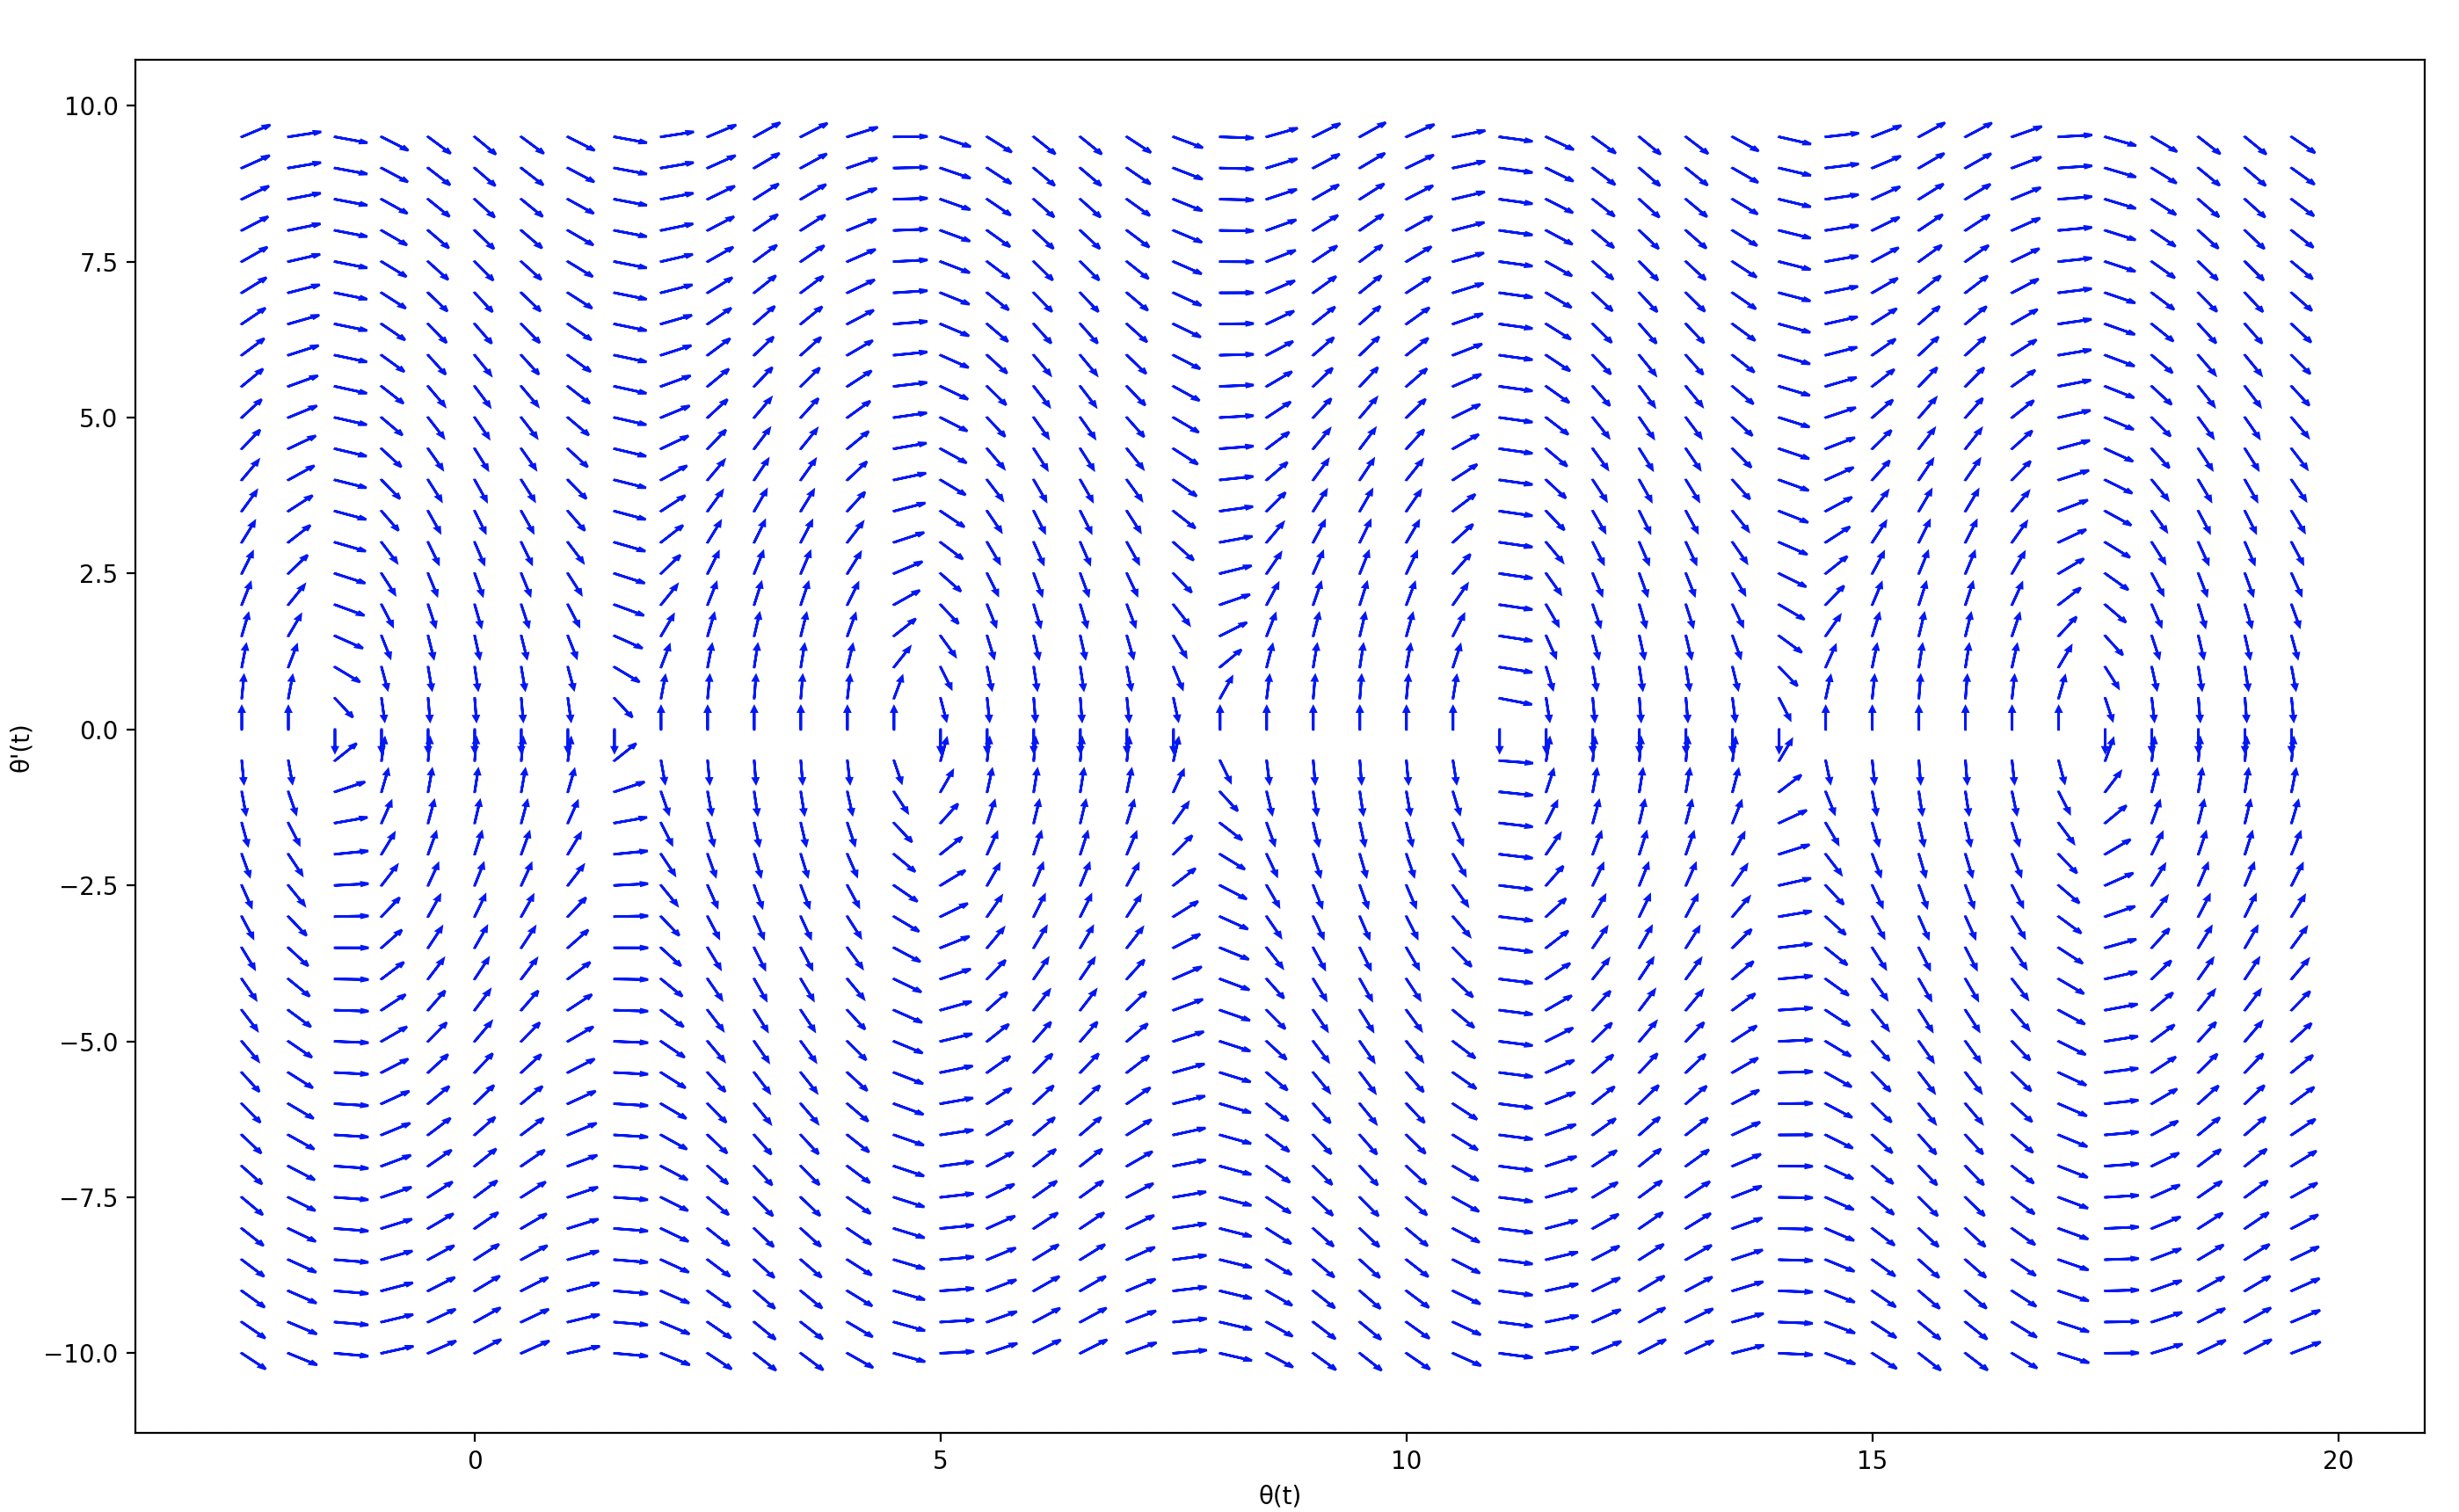
\includegraphics[width=1.4\textwidth]{undertorqued problem.png}}%
  \caption{Vector field of a pendulum}
  \label{fig:key}
\end{figure}


\section{The robot arm}
\centering This section covers the derivation and simulation of the equations of motion for an arm with an arbitrary number of joints. The robot arm is modeled as a collection of 1-joint problems organized sequentially:

\vspace{24pt}

\centering 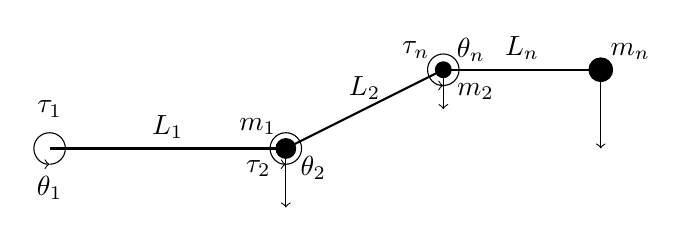
\begin{tikzpicture}


% Draw the lines
  \draw[thick] (0,0) -- (3,0);
  \draw (1.5,0) node[anchor=south] {$L_1$};
% Draw the dots
  \filldraw (3,0) circle (0.125cm);
  \draw (3,0.05) node[anchor=south east] {$m_1$};
%gravity vector
    \draw[->] (3,0) -- (3, -0.75);
% Draw the arcs and torques
  \draw[->] (0, -0.2) arc (-90:270:0.2cm);
  \draw (0, 0.5) node {$\tau_1$};
  \draw (0, -0.5) node {$\theta_1$};


   \draw[thick] (3,0) -- (5,1);
  \draw (4, 0.5) node[anchor=south] {$L_2$};
    \filldraw (5,1) circle (0.1cm);
  \draw (5.05,0.5) node[anchor=south west] {$m_2$};
    \draw[->] (5,1) -- (5, 0.5);
\draw[->] (3, -0.2) arc (-90:270:0.2cm);
  \draw (2.65, -0.25) node {$\tau_2$};
  \draw (3.35, -0.25) node {$\theta_2$};

  

\draw[thick] (5,1) -- (7,1);
\draw (6, 1) node[anchor=south] {$L_n$};
\filldraw (7,1) circle (0.15cm);
\draw (7,1) node[anchor=south west] {$m_n$};
\draw[->] (7,1) -- (7, 0);
\draw[->] (5, 0.8) arc (-90:270:0.2cm);
  \draw (4.65, 1.25) node {$\tau_n$};
  \draw (5.35, 1.25) node {$\theta_n$};

  %draw gravity arrow
\end{tikzpicture}

\vspace{14pt}
\noindent \justifying Note that $\tau_1 = \tau_1(t)$, time dependencies have been removed for simplicity. 
\vspace{14pt}

\subsection{Deriving the equations of motion for an arbitrary number of sequential 1-joint problems}

\paragraph{Rotational Inertia} Finding the rotational inertia and the torque exerted by gravity becomes complicated when more joints are involved. These quantities need to be computed with respect to each joint. For joint a in the system:

\vspace{24pt}
\centering $I_a = m_nL_{a,mn}^2 + m_{n-1}L_{a,mn-1}^2 ... + m_aL_a^2$ ,
\vspace{24pt}

\noindent \justifying where $I_a$ is the inertia calculated with respect to joint A, and $L_{a,mn}$, is the distance from joint a to the last mass. $L_{a,mn-1}$ is the distance from joint a to the second last mass. Only masses past the joint count toward its rotational inertia. The lengths used in the inertia formula are computed by treating the 1 joint problems downstream of the joint as  vectors of magnitude $L_i$ and direction $\theta_i$. These vectors can be summed to calculate the net vector. The vector below is computed from joint a (which we're calculating the inertia WRT to) to joint b, a joint we're trying to find the distance to. 

\vspace{24pt}
\centering $\vec{v}_{a,b} = J_a + J_{a+1} + ... + J_b$,
\vspace{14pt}

\indent where $J_a =  \begin{bmatrix} L_acos(\theta_a) \\ L_asin(\theta_a) \end{bmatrix}$ 
 \hspace{1cm}   $|\vec{v}_{a,b}| = L_{a,b}$  \hspace{1cm} $\hat v_{a,b} = \theta_{a,b}$
 \vspace{24pt}
 \newpage

The rotational inertia with respect to a joint in the system can be computed from this.

\vspace{24pt}
\centering $I_a = m_n|\vec{v}_{a,n}|^2 + m_{n-1}|\vec{v}_{a,n-1}|^2 + ... + m_AL_A^2$
\vspace{14pt}


\paragraph{torque applied by gravity} 
With the quantities just developed, the torque applied by gravity WRT to joint a can be computed:
\vspace{24pt}

$\tau_a = m_a*L_{a}*cos(\theta_a)*g + m_{a+1}*L_{a,a+1}*cos(\theta_{a,a+1})*g + ... + m_{b}*L_{a,b}*cos(\theta_{a1,b})*g$

\vspace{24pt}

\paragraph{Equations of motion} 
\noindent \justifying The equations of motion of this system are a $2n$th order differential equation. Since this equation is nonlinear, its matrix form is quite messy. It will instead be written as a system of first-order equations:

\vspace{24pt}
\centering $\theta_1 = y_1  \hspace{0.5cm}  \theta_1' = y_2  \hspace{0.5cm}  \theta_2 = y_3  \hspace{0.5cm}  \theta_2' = y_4 \hspace{0.5cm} ....\hspace{0.5cm} \theta_n = y_{2n-1} \hspace{0.5cm} \theta_n' = y_{2n}$

\vspace{24pt}
\noindent \justifying $m_1gLcos(y_1)$ and ${m_1L^2}$ used in the 1-joint problem are now $\tau_1$ and $I_1$, which are functions of $\theta_1, \theta_2, ..., \theta_n$
\vspace{24pt}

\centering$y_1' = y_2$   \hspace{1cm}  $y_2' = \frac{\tau_{app1}(t) - \tau_1}{I_1} - By_2$ 

\vspace{10pt}

\centering$y_3' = y_4$   \hspace{1cm}  $y_4' = \frac{\tau_{app2}(t) - \tau_2}{I_2} - By_4$

\vspace{10pt}

\centering $...$

\vspace{10pt}

\centering$y_{2n-1}' = y_{2n}$   \hspace{1cm}  $y_{2n}' = \frac{\tau_{appn}(t) - \tau_n}{I_n} - By_{2n}$ \\ 

\vspace{24pt}

\newpage 

\subsection{Programming and simulating the robot arm}

\noindent \justifying A function that calculates the rotational inertia and torque applied by gravity with respect to each joint is defined:
\vspace{24pt}
\begin{lstlisting}[language=Python]
def slopes(t, Input):     # Y is a vector of shape [x1, x2,..., xn]
    output = np.zeros(sn*2)

    #computes the distance between joints in an arm
    for joint_computed in range(sn):  #iterate joints
        rotational_inertia = 0 #rotational inertia WRT curr. joint
        net_torque_on_joint = 0 #net torque WRT curr joint
        for mass_computed in range((sn-1),(joint_computed-1),-1):
            lx, ly = 0, 0
            dist = 0
            #the vector sum
            for y in range(joint_computed, (mass_computed + 1)):
                lx = lx + Lengths[y]*np.cos(Input[y*2])
                ly = ly + Lengths[y]*np.sin(Input[y*2])
            dist = np.sqrt(lx**2 + ly**2) #The distance from Joint A to B   
            #The rotational inertia of the point mass computed is added to the system:
            rotational_inertia += Masses[mass_computed] * dist**2 
            net_torque_on_joint += Masses[mass_computed]*grav*dist*(lx/dist) 
            # lx/dist = adj/hyp = cos
        #take the inertia and torques calculated, and use them to compute the ODE:
        output[joint_computed*2] = Input[2*joint_computed + 1]
        output[joint_computed*2 +1] = ((Torques[joint_computed] - net_torque_on_joint) / rotational_inertia)  - Bs[joint_computed]*Input[2*joint_computed + 1] #x2'
    return(output)
    
\end{lstlisting}
Note: sn is the number of segments in the arm

\newpage
\vspace{24pt}
\noindent \justifying The simulation parameters are now vectorized, and they can be of an arbitrary length:
\vspace{24pt}

\begin{lstlisting}[language=Python]
sn = 4

Lengths = [2, 1, 0.75, 2] # lenghths (m)
Bs = [0.5, 0.5, 0.5, 0.25] # friction terms 
Masses = [3, 5, 1, 3] # mass terms (kg)
Torques = [300, 3, 50, 5] # torque terms (Nm)
Init_values = [0.1,0.3,0.1,0.3,0.1,0.3,0,0] # position1, velocity1, position2, velocity2, ....., positionn, velocityn

grav = 9.81
simulationDuration = 20 # seconds
\end{lstlisting}

\vspace{24pt}

The animation code is very similar to the 1-joint problem. The full code can be found \textcolor{blue}{\href{https://github.com/natebechard/Robotic-Arm-Simulation-From-First-Principles/blob/main/n_joints_constant_torque.py}{here}}

\subsection{Simulations}
The n-joint arm exhibits interesting behavior. It can be played with extensively using the source code \textcolor{blue}{\href{https://github.com/natebechard/Robotic-Arm-Simulation-From-First-Principles/blob/main/n_joints_constant_torque.py}{here}}

- Inertia demo
- double and triple pendulums

\section{Experiment Ideas}
- Torque as a function
- let the joints act as an arm
- Nick's DC motor integrated in the ODE

\section{Conclusion}
\noindent \justifying The dynamics of a robot arm can be deconstructed into simple one-joint problems, which are 2nd order differential equations derived from basic laws of physics. The simulation of an arm is a demonstration of how a model based on basic laws, such as $F = ma$ and $\tau_g = mgrsin(\theta)$ can generate intricate emergent behavior. To a reader entering the field of engineering, this paper demonstrates a transition from rudimentary mathematical formulas, with no clear use in the real world, to real-world models that deepen our understanding of the universe. This will hopefully reveal the beauty of mathematics to hobbyists and makers. 

\centering \section{References}
\centering To discuss with teacher

\end{document}
